\chapter{Introduction}
\label{ch:intro}

The opening chapter of a thesis or dissertation will typically provide an introduction to the body of research. At the beginning of a chapter, it is common to provide some introductory text. Instead of discussing research, this template document will highlight how the {\ttfamily byuthesis.cls} \LaTeX{} class can be used to prepare a thesis or dissertation document for submission in the College of Engineering at BYU.

\section{Styles}
\label{sec:intro_styles}
The formatting and \LaTeX{} features that you will use to prepare your thesis are outlined briefly in the next several chapters. The narrow, single column format of this document is based on long-standing principles of typography~\cite{Bringhurst19}. This formatting is easy to read compared to the wide-column, double-spaced format used previously. The format of the document is defined in {\ttfamily byuthesis.cls}, a \LaTeX{} class defined specifically for theses and dissertations in the College of Engineering at BYU. To give a better sense of the format of the document, we will occasionally throw in some random Latin text to take up white space. We set it apart from the text requiring your attention with a grey font color.

{\color{mediumgray} \blindtext}

This is an example of a sentence with a footnote.\footnote{This is a footnote.} You can make a reference to a section by using its label, such as~\cref{sec:intro_styles}. You can reference a chapter in this way, for example~\cref{ch:intro}. Here is an example of a citation of a master's thesis~\cite{masters1}. References for this template document are held in a file called {\ttfamily references.bib}.

\subsection{Including Figures and Tables}
The syntax above provides an example for declaring a subsection. This subsection will include some text and give an example of a figure and a table. Let's start with with a figure. Figure~\ref{fig:gradf_half_space} shows the gradient of a function and the halfspace where the function is decreasing. Notice how the \verb|\ref| command automatically references the correct figure number. Notice also that the \verb|~| inserts a non-breaking space, so that the label Figure and the figure number are never separated by a line break.

\begin{figure}[htbp]
	\centering
	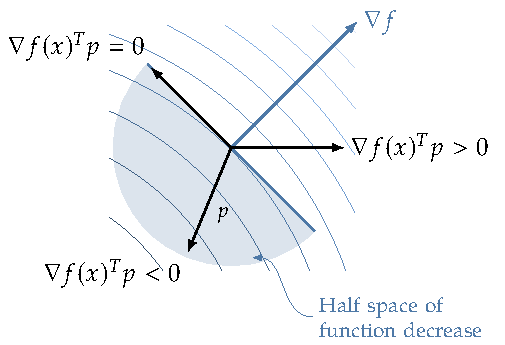
\includegraphics[width=3.0in]{figures/gradf_half_space}
	\caption{This is a regular figure.}
	\label{fig:gradf_half_space}
\end{figure}

{\color{mediumgray} \blindtext}

\subsubsection{Subsubsection Example}
The syntax above provides an example of how to include a subsubsection. In this thesis template, the document has four primary division levels: \verb|\chapter|, \verb|\section|, \verb|\subsection|, and \verb|\subsubsection|. The command \verb|\subsubsection| is used to define the lowest level of division. Notice that subsubsection titles are not numbered.

\subsubsection{Including Tables}
Tables are also fairly straightforward to include in a \LaTeX{} document. Table~\ref{tab:table_example} shows a simple table. \LaTeX{} refers to figures and tables as floats and often tries to locate figures at the top or bottom of a page. The user has some control over this, but \LaTeX{} can behave like it has a mind of its own sometimes. In reality it is placing figures according to internal algorithms and parameters that you can adjust. If you are interested in digging into this level of detail, an internet search on ``LaTeX float parameters'' will provide ample reading.

\begin{table}
	\centering
	\begin{tabular}{ c c c c}
		\toprule
		basin & curve \\
		name & number & minimum & maximum \\
		\midrule
		1B & 68.5 & 49.2 & 84.1 \\ 
		2B & 66.2 & 46.8 & 82.7\\ 
		3B & 65.4 & 45.5 & 82.3\\
		\midrule
		average & 66.7 & 47.2 & 83.0\\
		\bottomrule
	\end{tabular}
	\caption{This is a standard table with a top caption.}
	\label{tab:table_example}
\end{table}

\subsection{Formatting Equations}
Equation formatting is one of \LaTeX's most useful features and a good reason why it is often used for theses and dissertations in the College of Engineering. It is easy to format equations within a sentence, such $c = 2 \pi r$ to describe the circumference of a circle. Equations should be treated as part of the text. As an example, the surface area of a cylinder is given by
\begin{equation}
	\label{eq:surface_area_cyl}
	S = 2\pi r \left( r + h \right) ,
\end{equation}
where $r$ is the radius of the cylinder and $h$ is its height. The area of a circle can be expressed in terms of its diameter $d$ as 
\begin{equation}
	\label{eq:area_circle}
	A = \frac{\pi}{4} d^2 .
\end{equation}

Often, it is desirable to align a sequence of equations. Again, \LaTeX{} makes this pretty easy. The roots of the polynomial function $f(x)$ can be found by factoring
\begin{align}
	f(x) &= x^3 + 5x^2 + 6x \\
		 & = x (x^2 + 5x + 6) \\
		 & = x (x + 2)(x +3) ,
\end{align}
setting each of the factors to zero, and solving for $x$. Equations without numbers can be typeset like this
\[
	x = a + b
\]
or like this
\begin{equation*}
	y = c + d .
\end{equation*}
Just as we did with sections, figures, and tables, we can reference a specific equation by using its declared label. In~\eqref{eq:surface_area_cyl}, the surface area of a cylinder is defined. Another format would be to say Equation~\ref{eq:area_circle} defines the area of a circle. Yet another format is \cref{eq:area_circle}. Any of these formats is acceptable. Use just one of them and be consistent.
